\subsection{Hệ thống tóm tắt đa tầng hỗ trợ truy xuất và tìm kiếm thông tin}

Trong các hệ thống xử lý hội thoại dài như transcript cuộc họp, việc truy xuất trực tiếp trên toàn bộ dữ liệu gốc thường gặp nhiều khó khăn do kích thước văn bản lớn, mật độ thông tin không đồng đều và sự tồn tại của nhiều đoạn hội thoại mang ít giá trị ngữ nghĩa. Các cuộc họp thực tế thường chứa nhiều câu xác nhận ngắn, trao đổi mang tính điều phối hoặc các đoạn lặp lại nội dung đã được đề cập trước đó. Nếu toàn bộ transcript đều được sử dụng trực tiếp cho indexing và retrieval, chi phí xử lý sẽ tăng đáng kể trong khi hiệu quả truy xuất không tương ứng.

Để giải quyết vấn đề này, hệ thống xây dựng cơ chế tóm tắt đa tầng nhằm tổ chức lại thông tin theo nhiều mức độ ngữ nghĩa khác nhau. Thay vì chỉ sinh ra một bản tóm tắt duy nhất cho toàn bộ cuộc họp, hệ thống phân tách dữ liệu thành nhiều tầng biểu diễn, trong đó mỗi tầng tập trung vào một mức thông tin riêng biệt. Cách tiếp cận này giúp giảm đáng kể kích thước dữ liệu cần xử lý nhưng vẫn duy trì khả năng bảo toàn nội dung quan trọng phục vụ retrieval và semantic search.

Kiến trúc của hệ thống gồm bốn tầng chính bao gồm transcript layer, participant layer, topic layer và meeting layer. Các tầng này tạo thành một cấu trúc biểu diễn phân cấp, cho phép hệ thống duy trì cả thông tin chi tiết ở mức hội thoại lẫn khả năng biểu diễn ngữ nghĩa cô đọng ở mức tổng quát hơn.

\begin{figure}[H]
    \centering
    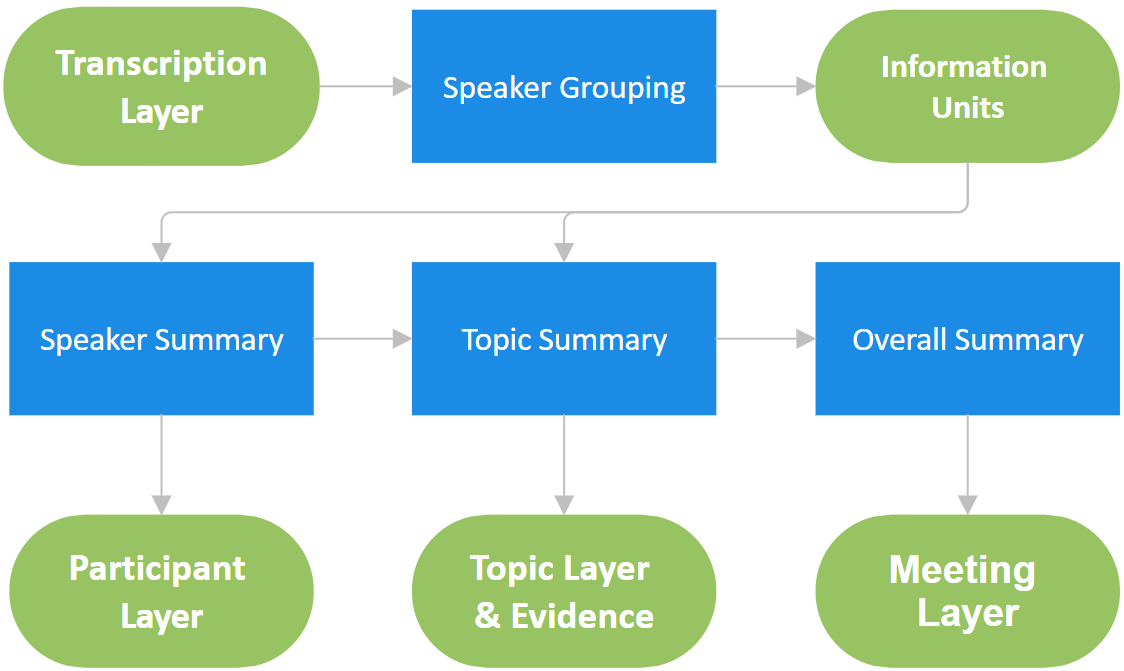
\includegraphics[width=\textwidth]{images/multisummary.png}
    \caption{Kiến trúc hệ thống tóm tắt đa tầng hỗ trợ truy xuất và tìm kiếm thông tin}
    \label{fig:multisummary_architecture}
\end{figure}

\subsubsection{Transcript Layer}

Transcript layer là tầng dữ liệu gốc của hệ thống và đóng vai trò lưu trữ toàn bộ nội dung hội thoại sau quá trình xử lý audio. Tầng này được xây dựng từ kết quả của pipeline speech recognition và speaker diarization, bao gồm các bước nhận dạng giọng nói, ghép speaker segments, chuẩn hóa văn bản và tái tạo transcript hoàn chỉnh của cuộc họp.

Mỗi đoạn transcript chứa thông tin về speaker, thời gian bắt đầu, thời gian kết thúc và nội dung phát biểu tương ứng. Đây là tầng có mức độ chi tiết cao nhất và phản ánh đầy đủ diễn biến thực tế của cuộc họp.

Tuy nhiên, transcript gốc thường có kích thước rất lớn và chứa nhiều đoạn hội thoại không mang nhiều giá trị truy xuất như các câu xác nhận ngắn, trao đổi mang tính điều phối hoặc các nội dung lặp lại. Việc sử dụng trực tiếp toàn bộ transcript cho retrieval sẽ làm tăng chi phí indexing và similarity search, đặc biệt khi số lượng cuộc họp tăng lên.

Vì vậy, transcript layer chủ yếu được sử dụng như nguồn dữ liệu gốc phục vụ đối chiếu và xác minh thông tin khi cần truy cập ngữ cảnh chi tiết. Đây cũng là tầng cuối cùng giúp hệ thống truy xuất lại đầy đủ nội dung hội thoại thay vì chỉ các biểu diễn cô đọng ở mức tóm tắt.

\subsubsection{Participant Layer}

Participant layer là tầng tóm tắt được tổ chức theo từng người tham gia trong cuộc họp. Mục tiêu của tầng này là xây dựng biểu diễn ngữ nghĩa tập trung vào đóng góp của từng speaker thay vì toàn bộ diễn biến hội thoại.

Hệ thống thực hiện gom nhóm các phát biểu theo speaker, sau đó trích xuất các information units quan trọng để tạo participant summaries cho từng người tham gia. Quá trình này tập trung giữ lại các nội dung mang giá trị thông tin cao như quyết định, đề xuất, yêu cầu, ràng buộc kỹ thuật hoặc trách nhiệm được giao trong cuộc họp.

Các câu mang tính hội thoại ngắn, xác nhận đơn giản hoặc lặp lại thường được loại bỏ nhằm tăng mật độ thông tin và giảm nhiễu trong dữ liệu tóm tắt. Điều này giúp participant summaries phản ánh rõ hơn vai trò và nội dung đóng góp của từng speaker thay vì lưu lại toàn bộ hội thoại nguyên bản.

Participant layer cho phép hệ thống nhanh chóng xác định người liên quan đến một chủ đề cụ thể hoặc truy vết các quyết định và đề xuất theo speaker. Ví dụ, hệ thống có thể xác định ai là người đề xuất một giải pháp, ai chịu trách nhiệm cho một tác vụ hoặc ai đã thảo luận về một yêu cầu kỹ thuật cụ thể.

So với transcript layer, participant layer có mức độ cô đọng cao hơn đáng kể nhưng vẫn giữ được khả năng biểu diễn thông tin ở mức chi tiết theo từng người tham gia. Đây là tầng trung gian quan trọng giúp giảm phạm vi tìm kiếm trước khi cần truy cập xuống transcript đầy đủ.

\subsubsection{Topic Layer}

Topic layer là thành phần trung tâm của hệ thống tóm tắt đa tầng và đóng vai trò biểu diễn nội dung ở mức ngữ nghĩa trung gian của cuộc họp. Khác với participant layer vẫn phụ thuộc vào speaker, topic layer tổ chức thông tin theo các chủ đề thảo luận thay vì theo người phát biểu.

Tầng này được xây dựng bằng cách gom nhóm các information units liên quan, kết hợp các đoạn hội thoại thuộc cùng chủ đề và tạo các topic summaries có mật độ thông tin cao hơn. Mỗi topic summary tập trung mô tả nội dung thảo luận chính, các quyết định quan trọng, ràng buộc kỹ thuật, yêu cầu thiết kế, các đánh đổi giữa nhiều lựa chọn và kết luận liên quan đến chủ đề đó.

Do không còn phụ thuộc vào cấu trúc hội thoại gốc theo speaker, topic summaries có khả năng biểu diễn ngữ nghĩa cô đọng hơn participant summaries trong khi vẫn giữ được phần lớn nội dung quan trọng của cuộc họp.

Topic layer đặc biệt phù hợp cho các tác vụ retrieval và semantic search ở quy mô lớn do khả năng biểu diễn nội dung ở mức chủ đề thay vì mức phát biểu đơn lẻ. Việc sử dụng topic summaries cũng giúp giảm đáng kể số lượng văn bản cần indexing và similarity matching so với transcript gốc.

Ngoài ra, tầng này còn hỗ trợ phát hiện các cuộc họp có nội dung tương tự hoặc các chủ đề xuất hiện lặp lại giữa nhiều tài liệu khác nhau. Trong kiến trúc tổng thể của hệ thống, topic layer đóng vai trò cầu nối giữa transcript chi tiết và meeting summaries ở mức tổng quát.

\subsubsection{Meeting Layer}

Meeting layer là tầng tóm tắt tổng quát nhất của toàn bộ cuộc họp. Không giống transcript layer được xây dựng trực tiếp từ hội thoại gốc, meeting summaries được sinh ra từ các topic summaries đã được cô đọng ở tầng trước đó.

Tầng này tập trung giữ lại các quyết định chính, mục tiêu của cuộc họp, các yêu cầu quan trọng, vấn đề nổi bật và các kết luận tổng quát. Nhờ được xây dựng trên nền topic summaries thay vì transcript đầy đủ, meeting layer đạt mức độ nén thông tin rất cao nhưng vẫn duy trì khả năng biểu diễn các nội dung cốt lõi của cuộc họp.

Meeting summaries giúp biểu diễn nhanh nội dung tổng quát của một cuộc họp mà không cần truy cập toàn bộ transcript chi tiết. Điều này đặc biệt hữu ích khi xử lý số lượng lớn tài liệu hoặc cần thực hiện indexing ở mức tổng quát.

So với các tầng còn lại, meeting layer có mức độ cô đọng cao nhất và đóng vai trò như lớp biểu diễn ngữ nghĩa tổng quan của toàn bộ tài liệu.

\subsubsection{Đặc điểm của hệ thống tóm tắt đa tầng}

Hệ thống được thiết kế theo hướng ưu tiên bảo toàn thông tin quan trọng thay vì tối đa hóa mức độ rút gọn văn bản bằng mọi giá. Trong bối cảnh retrieval và semantic search, việc làm mất các information units quan trọng thường gây ảnh hưởng lớn hơn so với việc giữ lại thêm một lượng nhỏ nội dung dư thừa.

Các prompt của hệ thống được xây dựng nhằm hạn chế hiện tượng hallucination và duy trì độ bám sát với transcript gốc. Thay vì paraphrasing mạnh hoặc sinh lại nội dung theo hướng tự do, hệ thống ưu tiên extraction và giữ nguyên các cụm từ quan trọng khi có thể. Cách tiếp cận này giúp tăng độ tin cậy của dữ liệu tóm tắt và giảm nguy cơ sinh ra các thông tin không tồn tại trong transcript ban đầu.

Ngoài chức năng rút gọn dữ liệu, các tầng tóm tắt còn đóng vai trò như các biểu diễn trung gian phục vụ retrieval và semantic indexing. Nhờ việc tổ chức thông tin theo nhiều mức độ ngữ nghĩa khác nhau, hệ thống có khả năng duy trì cả tính cô đọng lẫn khả năng truy xuất chi tiết trên các tập dữ liệu hội thoại lớn.